% =====================================================================
%  Capítulo 10 — Resolução numérica
%  Inserir antes da seção de exercícios.
% =====================================================================
\section{Resolução numérica}
\label{sec:cap09-numerica}

Este capítulo enunciou a fórmula do quadrupolo como estimativa dimensional e
descreveu o \emph{chirp} em palavras. Nenhuma das duas coisas é suficiente
para conectar a teoria com um sinal real. Aqui fechamos essa lacuna: a
constante da fórmula do quadrupolo é obtida derivando o momento de quadrupolo
e conferida contra a forma fechada; a evolução da frequência é integrada; e o
resultado é confrontado com dois sistemas medidos, PSR~B1913+16 e GW150914.
Trabalhamos em unidades SI, convertendo apenas na impressão.

\subsection{Python}

\programa[Anel de partículas nas duas polarizações, verificação da fórmula do quadrupolo, teste de Hulse--Taylor e inspiral de uma binária compacta.]{codigo/cap09\_ondas.py}

\subsubsection*{O anel de partículas}

A equação de desvio geodésico em gauge TT, com a onda propagando-se em $z$,
reduz-se a
\begin{equation}
  \rd{^{2}\xi^{i}}{t^{2}} = \frac{1}{2}\,\rd{^{2}h^{\rm TT}_{ij}}{t^{2}}\,\xi^{j},
  \qquad\text{cuja integral é}\qquad
  \xi^{i}(t) = \left(\delta^{i}{}_{j} + \tfrac12 h^{\rm TT}_{ij}\right)\xi^{j}(0).
  \label{eq:cap10-anel}
\end{equation}

\begin{atencao}
Em gauge TT as \emph{coordenadas} das partículas livres não mudam --- elas
estão em queda livre e permanecem em repouso coordenado. O que muda é a
distância própria entre elas. Dizer que a onda ``empurra'' as massas é a
imagem errada; dizer que ela altera a régua é a certa. A elipse desenhada
abaixo é o lugar geométrico dos pontos a distância própria constante, que é
exatamente o que o interferômetro mede.
\end{atencao}

\begin{figure}[htbp]
  \centering
  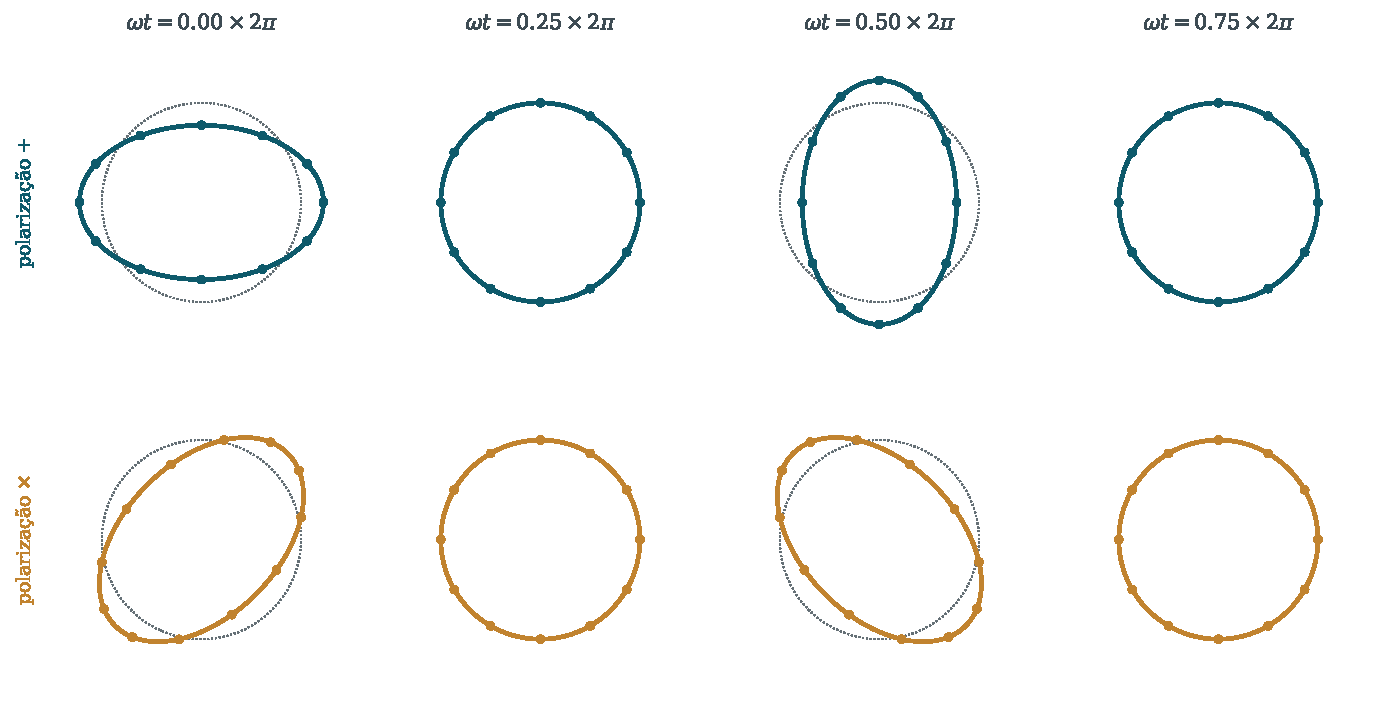
\includegraphics[width=\linewidth]{figuras/cap09_anel_polarizacoes.pdf}
  \caption{Deformação de um anel de partículas teste em quatro instantes de
  um período, para as duas polarizações (amplitude exagerada para
  $h=0{,}45$; o valor real é $10^{-21}$). O anel pontilhado é a
  configuração sem onda. A polarização $\times$ produz exatamente o mesmo
  padrão da $+$, girado de $45^\circ$ --- e não uma deformação de tipo
  novo. Em $\omega t = \pi/2$ e $3\pi/2$ o anel volta a ser circular: a onda
  não desloca as partículas em média, apenas oscila a distância entre elas.}
  \label{fig:cap10-anel}
\end{figure}

\subsubsection*{A fórmula do quadrupolo}

O texto deu apenas a escala $P\sim (G/c^{5})(\dddot Q)^{2}$. A expressão
completa é
\begin{equation}
  P = \frac{G}{5c^{5}}\left\langle \dddot Q_{ij}\,\dddot Q^{ij}\right\rangle,
  \qquad
  Q_{ij} = \mu\left(x_{i}x_{j} - \tfrac13\delta_{ij}r^{2}\right),
  \label{eq:cap10-quadrupolo}
\end{equation}
com $\mu = m_{1}m_{2}/(m_{1}+m_{2})$ a massa reduzida e $Q_{ij}$ o quadrupolo
\emph{sem traço}. Para testar a constante $1/5$ e o fator $32/5$ da forma
fechada, derivamos $Q_{ij}$ numericamente por um estêncil de sete pontos e
comparamos.

\begin{saida}
\begin{lstlisting}[style=rgsaida]
    a [km]    P numerico [W]     P fechado [W]   erro rel.
    100000      1.755723e+30      1.755723e+30    1.14e-07
   1000000      1.755723e+25      1.755723e+25    1.14e-07
  10000000      1.755723e+20      1.755723e+20    1.14e-07

-- para comparacao, o sistema Terra-Sol --
P (Terra-Sol) = 196.4 W   (a luminosidade do Sol e' 3.8e26 W)
\end{lstlisting}
\end{saida}

O erro de $10^{-7}$ é o truncamento do estêncil, não física: ele é o
\emph{mesmo} nas três linhas, enquanto a potência varia por dez ordens de
grandeza. Isso é o que se espera quando a expressão fechada está certa e a
discrepância vem só da derivada numérica.

\begin{central}
O sistema Terra--Sol irradia $196\,$W em ondas gravitacionais --- a potência
de algumas lâmpadas. A luminosidade eletromagnética do Sol é
$3{,}8\times10^{26}\,$W, mais de $10^{24}$ vezes maior. O fator $c^{5}/G
\approx 3{,}6\times10^{52}\,$W na fórmula é uma potência gigantesca dividindo
tudo: só massas relativísticas e compactas conseguem produzir algo
detectável. Não é que a gravidade ``não irradie''; é que a escala natural de
luminosidade gravitacional é absurdamente alta.
\end{central}

\subsubsection*{O teste de Hulse--Taylor}

Antes de qualquer detecção direta, a fórmula do quadrupolo já havia sido
verificada. Um sistema binário perde energia e o período orbital encolhe a
uma taxa que, para órbita excêntrica, é
\begin{equation}
  \rd{P_{b}}{t} = -\frac{192\pi}{5}
    \left(\frac{2\pi G}{P_{b}}\right)^{5/3}
    \frac{m_{1}m_{2}}{(m_{1}+m_{2})^{1/3}c^{5}}
    \frac{1 + \tfrac{73}{24}e^{2} + \tfrac{37}{96}e^{4}}{(1-e^{2})^{7/2}}.
  \label{eq:cap10-peters}
\end{equation}

\begin{saida}
\begin{lstlisting}[style=rgsaida]
dP_b/dt previsto pela RG  = -2.4031e-12
dP_b/dt observado (bruto) = -2.4230e-12
dP_b/dt observado, ja' descontada a aceleracao galactica = -2.3980e-12
razao previsto/observado = 1.0021
realce por excentricidade f(e) = 11.86   (orbita circular irradiaria 12x menos)
\end{lstlisting}
\end{saida}

Duas coisas merecem atenção. A primeira é a concordância de $0{,}2\,\%$ entre
uma fórmula deduzida de teoria linearizada e um pulsar a $6{,}4$~kpc --- o
resultado que rendeu o Nobel de 1993. A segunda é o desconto da aceleração
galáctica: o valor bruto medido difere do previsto em $0{,}8\,\%$, e a maior
parte dessa diferença não é falha da relatividade, mas o efeito Doppler
secular da aceleração relativa entre o sistema solar e o pulsar na Galáxia.
Comparar teoria com observação exige, quase sempre, remover primeiro efeitos
que nada têm a ver com o fenômeno estudado.

O fator $f(e) = 11{,}86$ explica por que esse sistema é tão bom laboratório:
com $e = 0{,}617$, ele irradia doze vezes mais que uma binária circular de
mesmo período, porque a emissão é fortemente concentrada na passagem pelo
periastro.

\subsubsection*{Inspiral e massa de chirp}

Igualando a perda de energia à variação da energia orbital newtoniana,
obtém-se uma equação para a frequência da onda, $f = 2f_{\rm orb}$:
\begin{equation}
  \rd{f}{t} = \frac{96}{5}\pi^{8/3}
  \left(\frac{G\mathcal{M}_{c}}{c^{3}}\right)^{5/3} f^{11/3},
  \qquad
  \mathcal{M}_{c} = \frac{(m_{1}m_{2})^{3/5}}{(m_{1}+m_{2})^{1/5}}.
  \label{eq:cap10-chirp}
\end{equation}

\begin{saida}
\begin{lstlisting}[style=rgsaida]
massa de chirp M_c = 28.10 M_sol
f_gw na ISCO       = 67.6 Hz
  f [Hz]   t ate coalescer [s]             h
      20                 0.845     5.549e-22
      35                 0.190     8.058e-22
      70                 0.030     1.279e-21
     130                 0.006     1.933e-21
integracao numerica de 20 Hz ate' a ISCO: 0.812 s
forma fechada (20 Hz -> infinito):        0.845 s
\end{lstlisting}
\end{saida}

Compare com o evento real: GW150914 entrou na banda do LIGO em torno de
$35$~Hz e durou cerca de $0{,}2$~segundo até a fusão, com amplitude de pico
próxima de $10^{-21}$. As três colunas reproduzem isso sem nenhum ajuste ---
massa de chirp, duração e amplitude saem todas da mesma equação de
primeira ordem.

\begin{figure}[htbp]
  \centering
  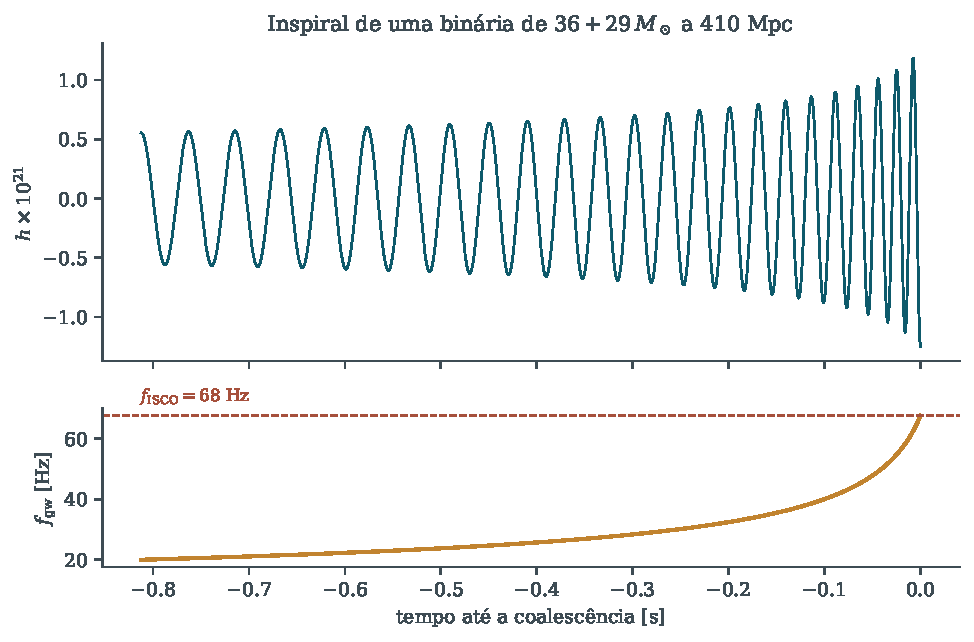
\includegraphics[width=\linewidth]{figuras/cap09_chirp.pdf}
  \caption{Acima, a forma de onda $h(t)$ da binária de $36+29\,\Msol$ a
  $410$~Mpc; abaixo, a frequência. Amplitude e frequência crescem juntas, e é
  daí que vem o nome \emph{chirp}. A integração para em
  $f_{\rm ISCO}=68$~Hz, onde a aproximação de órbita quase newtoniana deixa
  de valer e só a relatividade numérica descreve o que acontece.}
  \label{fig:cap10-chirp}
\end{figure}

\begin{central}
A frequência depende de $m_{1}$ e $m_{2}$ apenas pela combinação
$\mathcal{M}_{c}$. Essa é a razão física de a massa de chirp ser o parâmetro
mais bem medido em qualquer detecção: a fase do sinal, acumulada ao longo de
centenas de ciclos, a determina com precisão de poucos por cento, enquanto as
massas individuais só se separam por correções de ordem superior. Uma
degenerescência na teoria vira, na prática, uma hierarquia de incertezas
observacionais.
\end{central}

\subsection{Mathematica}

\programa[Linearização das equações de Einstein, gauge de Lorenz, onda plana em gauge TT e dedução exata do fator $32/5$.]{codigo/cap09\_ondas\_simbolico.wl}

O papel do cálculo simbólico aqui é o de derivar o que o numérico apenas
usa. O script parte de $g_{\mu\nu}=\eta_{\mu\nu}+\epsilon h_{\mu\nu}$, expande
o tensor de Ricci em primeira ordem e mostra que, no gauge de Lorenz, ele
colapsa no operador de onda.

Imposto $\partial^{\mu}\bar h_{\mu\nu}=0$, as equações de campo linearizadas
viram
\[
  \Box \bar h_{\mu\nu} = -16\pi G\,T_{\mu\nu},
\]
uma equação de onda com fonte, idêntica em estrutura à do potencial
eletromagnético em gauge de Lorenz. O segundo bloco confirma que a matriz TT
é solução, tem traço nulo e é transversal, e calcula a componente de
curvatura que entra no desvio geodésico, $R_{1010}=-\tfrac12\ddot h_{+}$.

Note que $\Box h^{\rm TT}=0$ vale para \emph{qualquer} par de funções
$h_{+}$ e $h_{\times}$ de $(t-z)$: a equação não escolhe uma forma de onda,
apenas exige que ela se propague à velocidade da luz sem dispersão. E
$R_{1010}=-\tfrac12\ddot h_{+}$ é a ponte com a
Equação~\eqref{eq:cap10-anel}: o que o detector mede é curvatura, não
deslocamento.

O último bloco deriva a Equação~\eqref{eq:cap10-quadrupolo} para a binária
circular sem nenhuma aproximação numérica: monta $Q_{ij}$ da órbita, deriva
três vezes em $t$ e simplifica, obtendo diretamente o fator $32/5$.

\begin{central}
O resultado simbólico e a derivação numérica concordam --- e é a combinação
das duas que constitui a verificação. O Mathematica prova que o fator é
exatamente $32/5$ para \emph{quaisquer} massas e separação; o Python
confirma, com números independentes, que a implementação usada para produzir
as figuras não tem erro de digitação. Nenhuma das duas checagens, sozinha,
faria esse trabalho.
\end{central}

